\documentclass{beamer}
\usepackage[utf8]{inputenc}
\usepackage{graphicx, epsfig}
\usepackage{amsmath,mathrsfs,amsfonts,amssymb}
%\usepackage{subfig}
\usepackage{floatflt}
\usepackage{epic,ecltree}
\usepackage{mathtext}
\usepackage{fancybox}
\usepackage{fancyhdr}
\usepackage{multirow}
\usepackage{enumerate}
\usepackage{epstopdf}
\usepackage{multicol}
\usepackage{algorithm}
\usepackage[noend]{algorithmic}
\usepackage{tikz}
\usepackage{blindtext}
\usetheme{default}%{Singapore}%{Warsaw}%{Warsaw}%{Darmstadt}
\usecolortheme{default}
\setbeamerfont{title}{size=\Huge}
\setbeamertemplate{footline}[page number]{}


\makeatletter
\newcommand\HUGE{\@setfontsize\Huge{35}{40}}
\makeatother    

\setbeamerfont{title}{size=\HUGE}
\beamertemplatenavigationsymbolsempty

% latin bold lower
\newcommand{\ba}{\mathbf{a}} 
\newcommand{\bc}{\mathbf{c}} 
\newcommand{\be}{\mathbf{e}} 
\newcommand{\bh}{\mathbf{h}} 
\newcommand{\bp}{\mathbf{p}} 
\newcommand{\bt}{\mathbf{t}} 
\newcommand{\bs}{\mathbf{s}} 
\newcommand{\bu}{\mathbf{u}} 
\newcommand{\bv}{\mathbf{v}} 
\newcommand{\bw}{\mathbf{w}} 
\newcommand{\bx}{\mathbf{x}} 
\newcommand{\by}{\mathbf{y}} 
\newcommand{\bz}{\mathbf{z}} 

% latin bold upper
\newcommand{\bA}{\mathbf{A}} 
\newcommand{\bB}{\mathbf{B}} 
\newcommand{\bC}{\mathbf{C}} 
\newcommand{\bI}{\mathbf{I}} 
\newcommand{\bL}{\mathbf{L}} 
\newcommand{\bM}{\mathbf{M}} 
\newcommand{\bQ}{\mathbf{Q}} 
\newcommand{\bT}{\mathbf{T}} 
\newcommand{\bU}{\mathbf{U}} 
\newcommand{\bV}{\mathbf{V}} 
\newcommand{\bW}{\mathbf{W}} 
\newcommand{\bX}{\mathbf{X}} 
\newcommand{\bY}{\mathbf{Y}} 
\newcommand{\bZ}{\mathbf{Z}} 

% latin cal upper
\newcommand{\cG}{\mathcal{G}} 
\newcommand{\cL}{\mathcal{L}} 
\newcommand{\cN}{\mathcal{N}} 
\newcommand{\cS}{\mathcal{S}} 
\newcommand{\cT}{\mathcal{T}} 
\newcommand{\cW}{\mathcal{W}} 
\newcommand{\cX}{\mathcal{X}} 
\newcommand{\cZ}{\mathcal{Z}} 

% latin bb upper
\newcommand{\bbE}{\mathbb{E}} 
\newcommand{\bbI}{\mathbb{I}} 
\newcommand{\bbP}{\mathbb{P}} 
\newcommand{\bbR}{\mathbb{R}} 

% greek bold lower
\newcommand{\bepsilon}{\boldsymbol{\epsilon}} 
\newcommand{\btheta}{\boldsymbol{\theta}} 
\newcommand{\blambda}{\boldsymbol{\lambda}} 
\newcommand{\bpi}{\boldsymbol{\pi}} 
\newcommand{\bmu}{\boldsymbol{\mu}} 
\newcommand{\bsigma}{\boldsymbol{\sigma}} 
\newcommand{\bphi}{\boldsymbol{\phi}} 

% greek bold upper
\newcommand{\bSigma}{\boldsymbol{\Sigma}} 

\DeclareMathOperator*{\argmin}{arg\,min}
\DeclareMathOperator*{\argmax}{arg\,max}

\newcommand{\createdgmtitle}[1]{\title[\hbox to 56mm{Deep Generative Models  \hfill\insertframenumber\,/\,\inserttotalframenumber}]
	{\vspace{1.5cm} \\ Deep Generative Models \\ {\Huge Lecture #1}}
	\author{Roman Isachenko}
	\institute{
	Moscow Institute of Physics and Technology
	} 
	\date{Autumn, 2021}
}

\newcommand\myfootnote[1]{%
  \tikz[remember picture,overlay]
  \draw (current page.south west) +(1in + \oddsidemargin,0.5em)
  node[anchor=south west,inner sep=0pt]{\parbox{\textwidth}{%
      \rlap{\rule{10em}{0.4pt}}\raggedright\scriptsize \textit{#1}}};}

\newcommand\myfootnotewithlink[2]{%
  \tikz[remember picture,overlay]
  \draw (current page.south west) +(1in + \oddsidemargin,0.5em)
  node[anchor=south west,inner sep=0pt]{\parbox{\textwidth}{%
      \rlap{\rule{10em}{0.4pt}}\raggedright\scriptsize\href{#1}{\textit{#2}}}};}
\createdgmtitle{3}
%--------------------------------------------------------------------------------
\begin{document}
%--------------------------------------------------------------------------------
\begin{frame}[noframenumbering,plain]
%\thispagestyle{empty}
\titlepage
\end{frame}
%=======
\begin{frame}{Recap of previous lecture}
	\begin{block}{MLE problem for autoregressive model}
		\vspace{-0.7cm}
		\[
		\btheta^* = \argmax_{\btheta} p(\bX | \btheta) = \argmax_{\btheta} \sum_{i=1}^n \sum_{j=1}^m \log p(x_{ij} | \bx_{i, 1:j - 1}\btheta).
		\]
		\vspace{-0.7cm}
	\end{block}
	\begin{block}{Sampling}
		\vspace{-0.5cm}
		\[
			\hat{x}_1 \sim p(x_1 | \btheta), \quad \hat{x}_2 \sim p(x_2 | \hat{x}_1, \btheta), \dots, \quad \hat{x}_m \sim p(x_m | \hat{\bx}_{1:m-1}, \btheta)
		\]
		New generated object is $\hat{\bx} = (\hat{x}_1, \hat{x}_2, \dots, \hat{x}_m)$.
	\end{block}
	Masking helps to make neural network autoregressive.
	\begin{itemize}
		\item \textbf{MADE} - masked autoencoder (MLP).
		\item \textbf{WaveNet} - masked 1D convolutions.
		\item \textbf{PixelCNN} - masked 2D convolutions.
	\end{itemize}
	\textbf{PixelCNN++} uses discretized mixture of logistic distribution to make the output distribution more natural.
\end{frame}
%=======
\begin{frame}{Recap of previous lecture}
	\begin{block}{Posterior distribution}
		\[
		p(\btheta | \bX) = \frac{p(\bX | \btheta) p(\btheta)}{p(\bX)} = \frac{p(\bX | \btheta) p(\btheta)}{\int p(\bX | \btheta) p(\btheta) d \btheta} 
		\]
		\vspace{-0.2cm}
	\end{block}
	\begin{block}{Bayesian inference}
		\vspace{-0.2cm}
		\[
		p(\bx | \bX) = \int p(\bx | \btheta) p(\btheta | \bX) d \btheta
		\]
		\vspace{-0.2cm}
	\end{block}
	\begin{block}{Maximum a posteriori (MAP) estimation}
		\vspace{-0.2cm}
		\[
		\btheta^* = \argmax_{\btheta} p(\btheta | \bX) = \argmax_{\btheta} \bigl(\log p(\bX | \btheta) + \log p(\btheta) \bigr)
		\]
		\vspace{-0.2cm}
	\end{block}
	\begin{block}{MAP inference}
		\[
		p(\bx | \bX) = \int p(\bx| \btheta) p(\btheta | \bX ) d \btheta \approx p(\bx | \btheta^*).
		\]
	\end{block}
\end{frame}
%=======
\begin{frame}{Latent variable models (LVM)}
	\begin{block}{MLE problem}
		\vspace{-0.5cm}
		\[
		\btheta^* = \argmax_{\btheta} p(\bX | \btheta) = \argmax_{\btheta} \prod_{i=1}^n p(\bx_i | \btheta) = \argmax_{\btheta} \sum_{i=1}^n \log p(\bx_i | \btheta).
		\]
		\vspace{-0.5cm}
	\end{block}
	The distribution $p(\bx | \btheta)$ could be very complex and intractable (as well as real distribution $\pi(\bx)$).
	\begin{block}{Extended probabilistic model}
		Introduce latent variable $\bz$ for each sample $\bx$
		\[
		p(\bx, \bz | \btheta) = p(\bx | \bz, \btheta) p(\bz); \quad 
		\log p(\bx, \bz | \btheta) = \log p(\bx | \bz, \btheta) + \log p(\bz).
		\]
		\[
		p(\bx | \btheta) = \int p(\bx, \bz | \btheta) d\bz = \int p(\bx | \bz, \btheta) p(\bz) d\bz.
		\]
	\end{block}
	\vspace{-0.3cm}
	\begin{block}{Motivation}
		The distributions $p(\bx | \bz, \btheta)$ and $p(\bz)$ could be quite simple.
	\end{block}
\end{frame}
%=======
\begin{frame}{Latent variable models (LVM)}
	\[
	\log p(\bx | \btheta) = \log \int p(\bx | \bz, \btheta) p(\bz) d\bz \rightarrow \max_{\btheta}
	\]
	\vspace{-0.6cm}
	\begin{block}{Examples}
		\begin{minipage}[t]{0.45\columnwidth}
			\textit{Mixture of gaussians} \\
			\vspace{-0.5cm}
			\begin{figure}
				\centering
				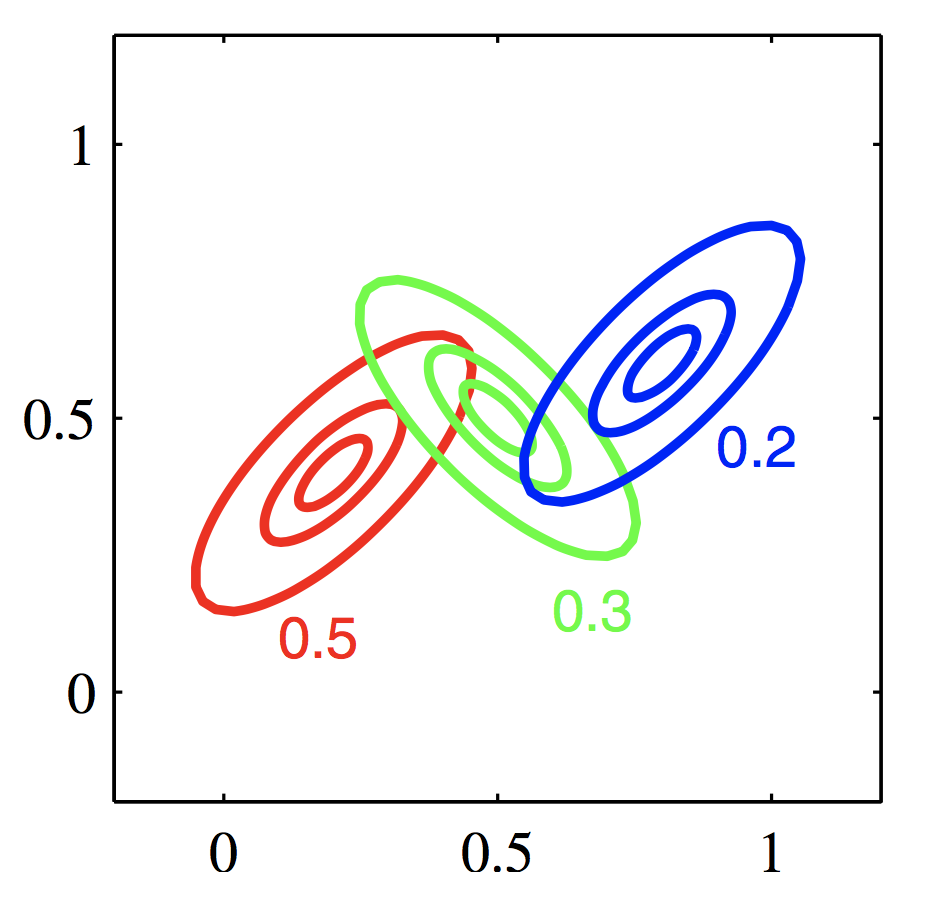
\includegraphics[width=0.75\linewidth]{figs/mixture_of_gaussians}
			\end{figure}
			\vspace{-0.5cm}
			\begin{itemize}
				\item $p(\bx | z, \btheta) = \cN(\bx | \bmu_z, \bSigma_z)$
				\item $p(z) = \text{Categorical}(\bpi)$
			\end{itemize}
		\end{minipage}%
		\begin{minipage}[t]{0.53\columnwidth}
			\textit{PCA model} \\
			\vspace{-0.5cm}
			\begin{figure}
				\centering
				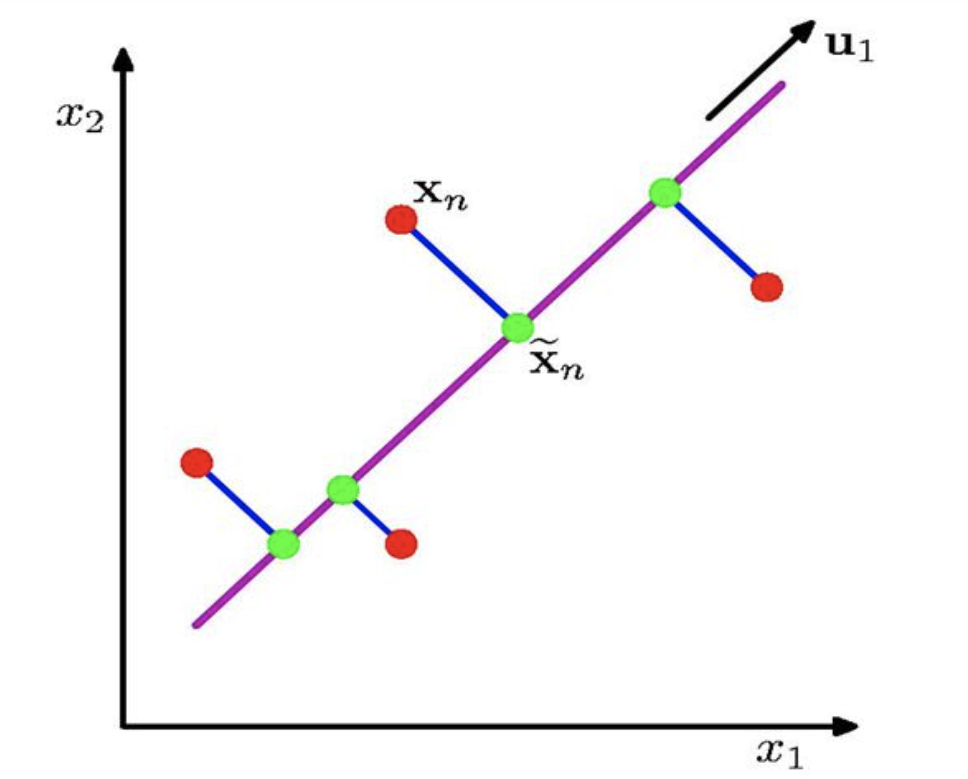
\includegraphics[width=.7\linewidth]{figs/pca}
			\end{figure}
			\vspace{-0.3cm}
			\begin{itemize}
				\item $p(\bx | \bz, \btheta) = \cN(\bx | \bW \bz + \bmu, \sigma^2 \bI)$
				\item $p(\bz) = \cN(\bz | 0, \bI)$
			\end{itemize}
		\end{minipage}
	\end{block}
	\myfootnote{Bishop\,C. Pattern Recognition and Machine Learning, 2006}
\end{frame}
%=======
\begin{frame}{Latent variable models (LVM)}
	\[
	\log p(\bx | \btheta) = \log \int p(\bx | \bz, \btheta) p(\bz) d\bz \rightarrow \max_{\btheta}
	\]
	\textbf{PCA} projects original data $\bX$ onto a low dimensional latent space while maximizing the variance of the projected data. 
	\begin{figure}
		\centering
		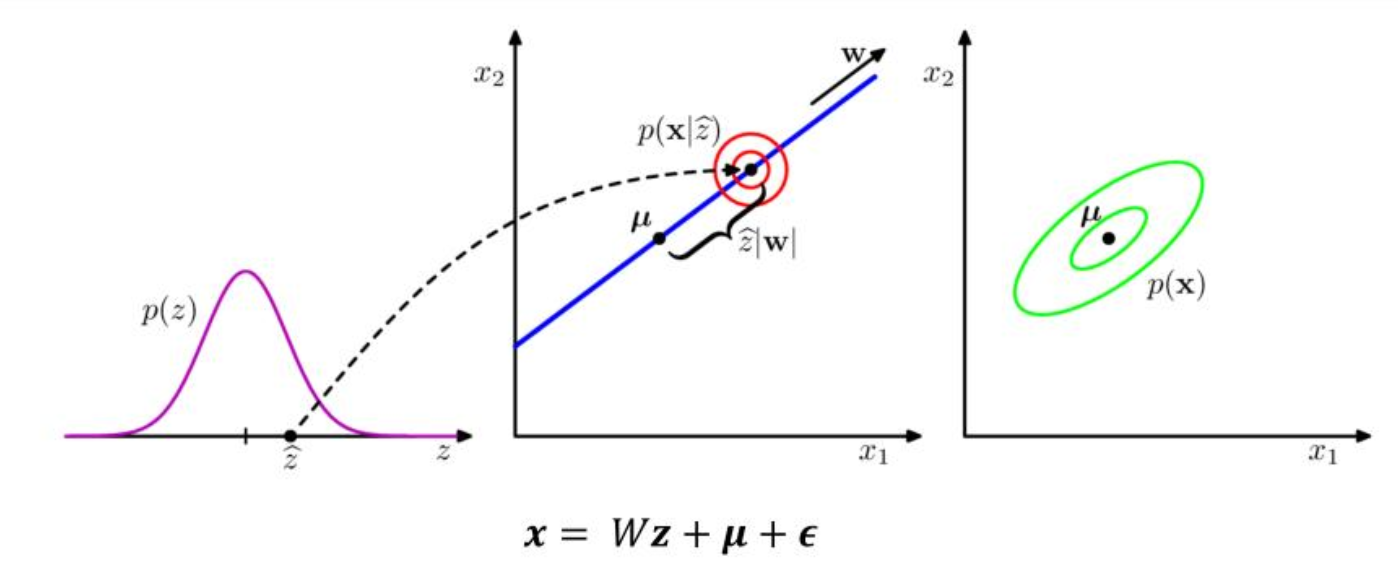
\includegraphics[width=.7\linewidth]{figs/bayesian_pca}
	\end{figure}
	\vspace{-0.5cm}
	\begin{itemize}
		\item $p(\bx | \bz, \btheta) = \cN(\bx | \bW \bz + \bmu, \sigma^2 \bI)$
		\item $p(\bz) = \cN(\bz | 0, \bI)$
		\item $p(\bx) = \cN(\bx | \bmu, \bW \bW^T + \sigma^2 \bI)$
		\item $p(\bz | \bx) = \cN \bigl(\bM^{-1} \bW^T (\bx - \bmu), \sigma^2 \bM\bigr)$, where $\bM = \bW \bW^T + \sigma^2 \bI$
	\end{itemize}
\end{frame}
%=======
\begin{frame}{Maximum likelihood estimation for LVM}
	\begin{block}{MLE for extended problem}
		\vspace{-0.7cm}
		\begin{multline*}
			\vspace{-0.5cm}
			\btheta^* = \argmax_{\btheta} p(\bX, \bZ | \btheta) = \argmax_{\btheta} \prod_{i=1}^n p(\bx_i, \bz_i | \btheta) = \\ = \argmax_{\btheta} \sum_{i=1}^n \log p(\bx_i, \bz_i | \btheta).
		\end{multline*}
		\vspace{-0.5cm}
	\end{block}
	However, $\bZ$ is unknown.
	\begin{block}{MLE for original problem}
		\vspace{-0.7cm}
		\begin{multline*}
			\btheta^* = \argmax_{\btheta} \log p(\bX| \btheta) = \argmax_{\btheta} \sum_{i=1}^n \log p(\bx_i | \btheta) = \\ =  \argmax_{\btheta}  \sum_{i=1}^n \log \int p(\bx_i, \bz_i | \btheta) d \bz_i = \\ = \argmax_{\btheta} \log \sum_{i=1}^n \int p(\bx_i| \bz_i, \btheta) p(\bz_i) d\bz_i.
		\end{multline*}
	\end{block}
	
\end{frame}
%=======
\begin{frame}{Naive approach}
	\begin{figure}
		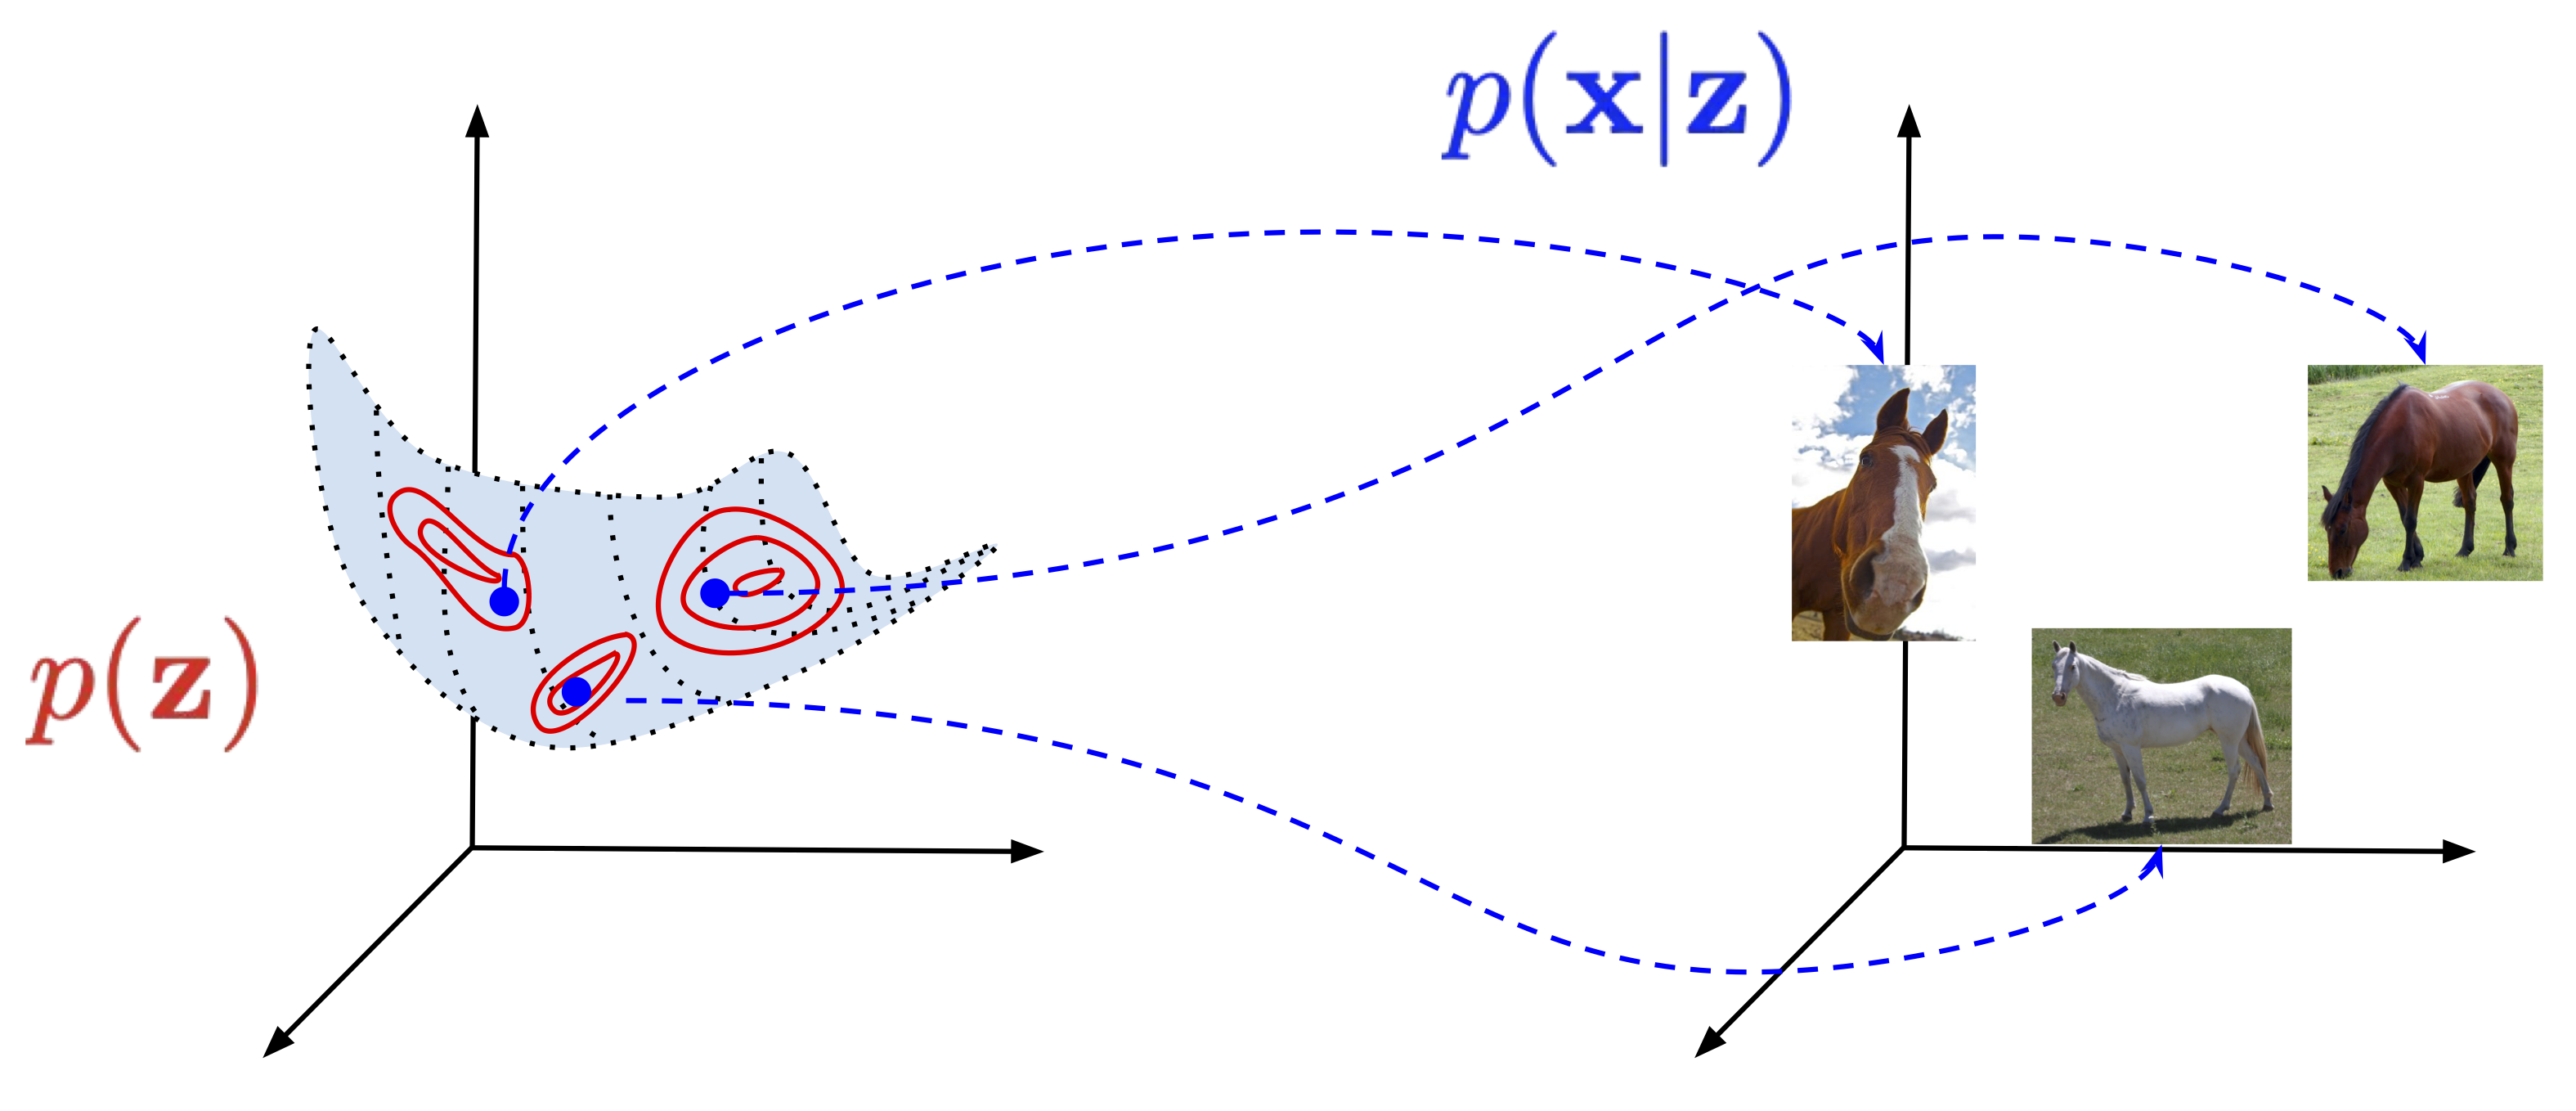
\includegraphics[width=.9\linewidth]{figs/lvm_diagram}
	\end{figure}
	\begin{block}{Monte-Carlo estimation}
		\vspace{-0.7cm}
		\[
			p(\bx | \btheta) = \int p(\bx | \bz, \btheta) p(\bz) d\bz = \bbE_{p(\bz)} p(\bx | \bz, \btheta) \approx \frac{1}{K} \sum_{k=1}^{K} p(\bx | \bz_k, \btheta)
		\]
		\textbf{Challenge:} to cover the space properly, the number of samples grows exponentially with respect to dimensionality of $\bz$. 
	\end{block}
	\myfootnotewithlink{https://jmtomczak.github.io/blog/4/4\_VAE.html}{image credit: https://jmtomczak.github.io/blog/4/4\_VAE.html}
\end{frame}
%=======
\begin{frame}{Variational lower bound}
	\begin{block}{Derivation 1}
		\vspace{-0.7cm}
		\begin{multline*}
			\log p(\bx| \btheta) 
			= \log \int p(\bx, \bz | \btheta) d\bz = \\ 
			= \log \int \frac{q(\bz)}{q(\bz)} p(\bx, \bz | \btheta) d\bz
			= \log \bbE_{q} \left[\frac{p(\bx, \bz| \btheta)}{q(\bz)} \right] \geq \\
			\geq \bbE_{q} \log \frac{p(\bx, \bz| \btheta)}{q(\bz)} = \int q(\bz) \log \frac{p(\bx, \bz| \btheta)}{q(\bz)} d \bz = \cL(q, \btheta)
		\end{multline*}
		\vspace{-0.7cm}
	\end{block}
	\begin{block}{Derivation 2}
		\vspace{-0.7cm}
		\begin{multline*}
			\log p(\bx| \btheta) 
			= \int q(\bz) \log p(\bx| \btheta) d\bz = \\ 
			= \int q(\bz) \log \frac{p(\bx, \bz| \btheta)}{p(\bz|\bx, \btheta)}d\bz
			= \int q(\bz) \log \frac{p(\bx, \bz| \btheta) q(\bz)}{p(\bz|\bx, \btheta) q(\bz)} d\bz = \\
			= \int q(\bz) \log \frac{p(\bx, \bz | \btheta)}{q(\bz)}d\bz + \int q(\bz) \log \frac{q(\bz)}{p(\bz|\bx, \btheta)}d\bz = \\ 
			= \mathcal{L} (q, \btheta) + KL(q(\bz) || p(\bz|\bx, \btheta)) \geq \mathcal{L} (q, \btheta).
		\end{multline*}
		\vspace{-0.7cm}
	\end{block}
\end{frame}
%=======
\begin{frame}{Variational lower bound}
	\begin{block}{Evidence Lower Bound (ELBO)}
		\vspace{-0.5cm}
		\begin{align*}
		    \mathcal{L} (q, \btheta) &= \int q(\bz) \log \frac{p(\bx, \bz | \btheta)}{q(\bz)}d\bz = \\ 
		    &= \int q(\bz) \log p(\bx | \bz, \btheta) d\bz + \int q(\bz) \log \frac{p(\bz)}{q(\bz)}d\bz \\ 
		    &= \mathbb{E}_{q} \log p(\bx | \bz, \btheta) - KL (q(\bz) || p(\bz))
		\end{align*}
		\vspace{-0.5cm}
	\end{block}
	\begin{block}{Log-likelihood decomposition}
		\vspace{-0.5cm}
		\[
			 \log p(\bx| \btheta) = \mathbb{E}_{q} \log p(\bx | \bz, \btheta) - KL (q(\bz) || p(\bz)) + KL(q(\bz) || p(\bz|\bx, \btheta)).
		\]
	\end{block}
	Instead of maximizing incomplete likelihood, maximize ELBO (equivalently minimize KL)
	\[
	    \max_{\btheta} p(\bx | \btheta) \quad \rightarrow \quad \max_{q, \btheta} \mathcal{L} (q, \btheta) \equiv \min_{q, \btheta} KL(q(\bz) || p(\bz|\bx, \btheta)).
	\]
	    
\end{frame}
%=======
\begin{frame}{EM-algorithm}
	\[
		\mathcal{L} (q, \btheta)  = \int q(\bz) \log p(\bx | \bz, \btheta) d\bz + \int q(\bz) \log \frac{p(\bz)}{q(\bz)}d\bz.
	\]
	\begin{block}{Block-coordinate optimization}
	\begin{itemize}
		\item Initialize $\btheta^*$;
		\item E-step
		\begin{multline*}
			q^*(\bz) = \argmax_q \mathcal{L} (q, \btheta^*) = \\
			= \argmin_q KL(q(\bz) || p(\bz | \bx, \btheta^*)) = p(\bz| \bx, \btheta^*);
		\end{multline*}
		\item M-step
		\[
			\btheta^* = \argmax_{\btheta} \mathcal{L} (q^*, \btheta);
		\]
		\item Repeat E-step and M-step until convergence.
	\end{itemize}
	\end{block}
\end{frame}
%=======
\begin{frame}{EM illustration}
	
	\begin{minipage}[t]{0.45\columnwidth}
		\begin{figure}
			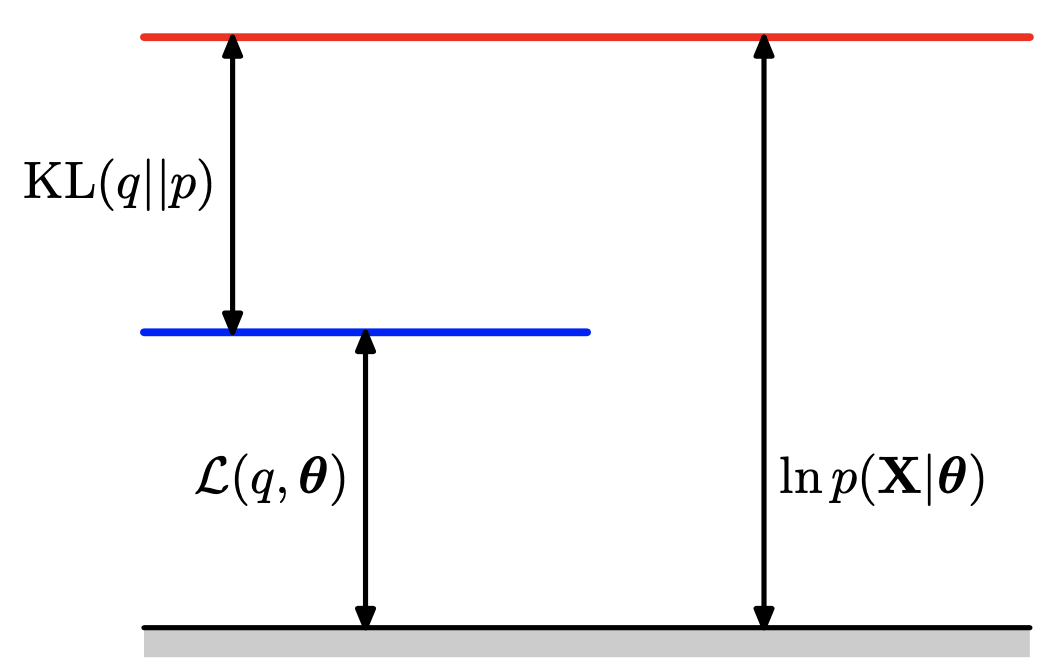
\includegraphics[width=0.9\linewidth]{figs/em_bishop1}
		\end{figure}
	\end{minipage}%
	\begin{minipage}[t]{0.55\columnwidth}
		\begin{figure}
			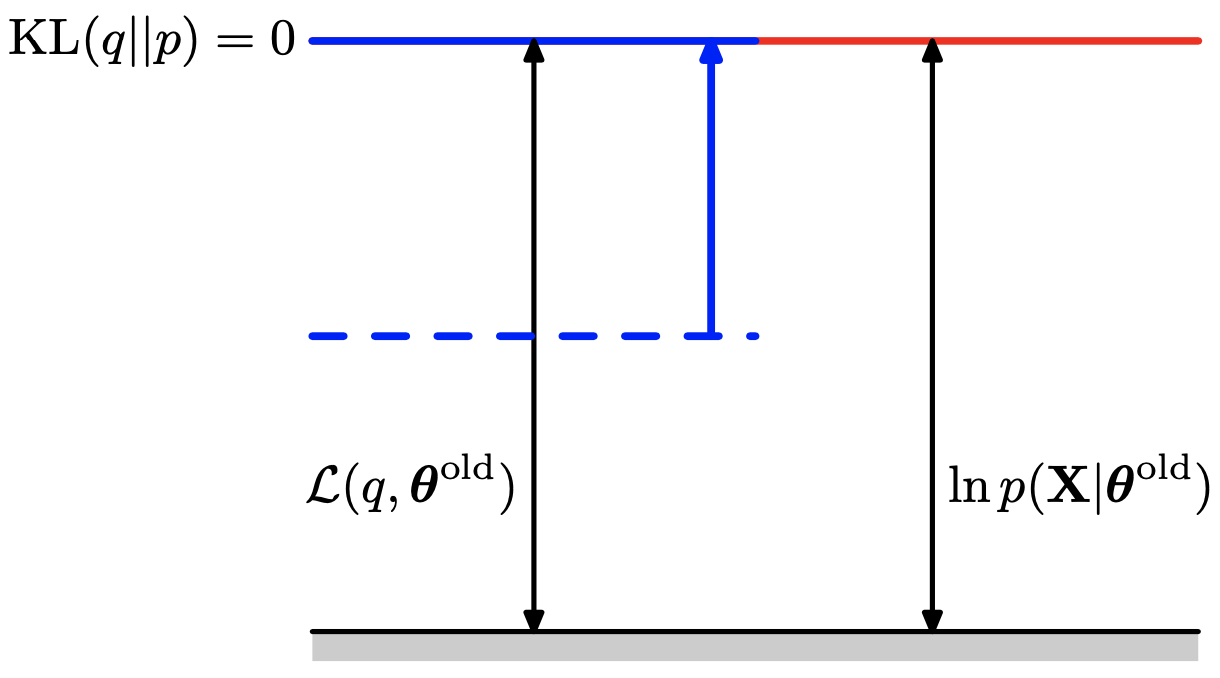
\includegraphics[width=0.85\linewidth]{figs/em_bishop2}
		\end{figure}
	\end{minipage}
	\begin{figure}
		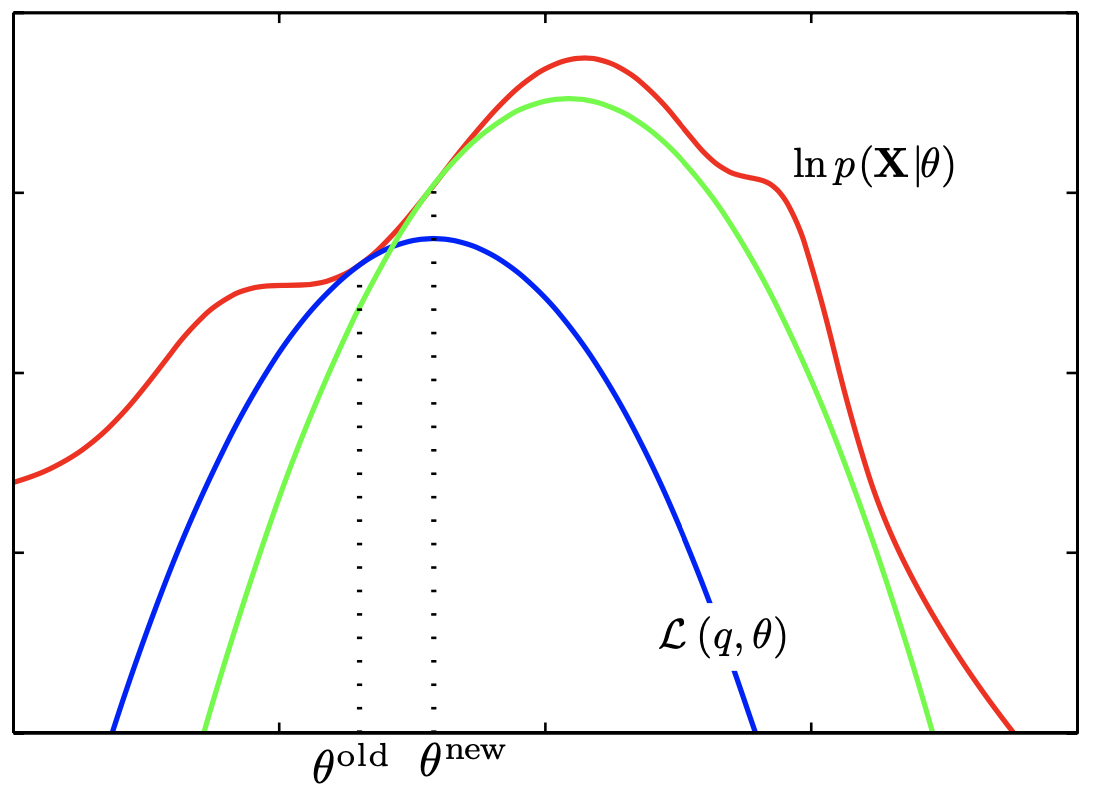
\includegraphics[width=.55\linewidth]{figs/em_bishop3}
	\end{figure}

	\myfootnote{Bishop\,C. Pattern Recognition and Machine Learning, 2006}
\end{frame}
%=======
\begin{frame}{Amortized variational inference}
    \begin{block}{E-step}
    \vspace{-0.3cm}
    \[
		q(\bz) = \argmax_q \mathcal{L} (q, \btheta^*) = \argmin_q KL(q || p) =
		 p(\bz| \bx, \btheta^*).
	\]
	\begin{itemize}
		\item $p(\bz| \bx, \btheta^*)$ could be \textbf{intractable};
		\item $q(\bz)$ is different for each object $\bx$.
	\end{itemize}
    \end{block}
	\begin{block}{Idea}
	Restrict a family of all possible distributions $q(\bz)$ to a parametric class $q(\bz|\bx, \bphi)$ conditioned on samples $\bx$ with parameters $\bphi$.
	\end{block}
	
	\textbf{Variational Bayes}
	\begin{itemize}
		\item E-step
		\[
		\bphi_k = \bphi_{k-1} + \left.\eta \nabla_{\bphi} \mathcal{L}(\bphi, \btheta_{k-1})\right|_{\bphi=\bphi_{k-1}}
		\]
		\item M-step
		\[
		\btheta_k = \btheta_{k-1} + \left.\eta \nabla_{\btheta} \mathcal{L}(\bphi_k, \btheta)\right|_{\btheta=\btheta_{k-1}}
		\]
	\end{itemize}
\end{frame}
%=======
\begin{frame}{Variational EM-algorithm}
	\begin{block}{ELBO}
		\vspace{-0.5cm}
		\[
			\log p(\bx| \btheta) = \mathcal{L} (\bphi, \btheta) + KL(q(\bz | \bx, \bphi) || p(\bz|\bx, \btheta)) \geq \mathcal{L} (\bphi, \btheta).
		\]
		\vspace{-0.5cm}
	\end{block}
	\begin{itemize}
		\item E-step
		\[
		\bphi_k = \bphi_{k-1} + \left.\eta \nabla_{\bphi} \mathcal{L}(\bphi, \btheta_{k-1})\right|_{\bphi=\bphi_{k-1}},
		\]
		where $\bphi$~-- parameters of variational distribution $q(\bz | \bx, \bphi)$.
		\item M-step
		\[
		\btheta_k = \btheta_{k-1} + \left.\eta \nabla_{\btheta} \mathcal{L}(\bphi_k, \btheta)\right|_{\btheta=\btheta_{k-1}},
		\]
		where $\btheta$~-- parameters of the generative distribution $p(\bx | \bz, \btheta)$.
	\end{itemize}
	Now all we have to do is to obtain two gradients $\nabla_{\bphi} \mathcal{L}(\bphi, \btheta)$, $\nabla_{\btheta} \mathcal{L}(\bphi, \btheta)$.  \\
	\textbf{Challenge:} Number of samples $n$ could be huge (we heed to derive unbiased stochastic gradients).
\end{frame}
%=======
\begin{frame}{ELBO gradients}
	\[
		 \mathcal{L} (\bphi, \btheta)  = \mathbb{E}_{q} \left[\log p(\bx | \bz, \btheta) + \log \frac{p(\bz)}{q(\bz | \bx, \bphi)} \right] \rightarrow \max_{\bphi, \btheta}.
	\]	
	\begin{block}{M-step: $\nabla_{\btheta} \mathcal{L}(\bphi, \btheta)$}
		\vspace{-0.7cm}
		\begin{multline*}
			\nabla_{\btheta} \mathcal{L} (\bphi, \btheta)
			= \int q(\bz|\bx, \bphi) \nabla_{\btheta}\log p(\bx|\bz, \btheta) d \bz \approx  \\
			\approx \nabla_{\btheta}\log p(\bx|\bz^*, \btheta), \quad \bz^* \sim q(\bz|\bx, \bphi).
		\end{multline*}
		\vspace{-0.7cm}
	\end{block}
	\begin{block}{E-step: $\nabla_{\bphi} \mathcal{L}(\bphi, \btheta)$}
	Difference from M-step: density function $q(\bz| \bx, \bphi)$ depends on the parameters $\bphi$, it is impossible to use the Monte-Carlo estimation:
	\begin{align*}
		\nabla_{\bphi} \mathcal{L} (\bphi, \btheta) &= \nabla_{\bphi} \int q(\bz | \bx, \bphi) \left[\log p(\bx | \bz, \btheta) + \log \frac{p(\bz)}{q(\bz| \bx, \bphi)} \right] d \bz \\
		& \neq  \int q(\bz | \bx, \bphi) \nabla_{\bphi} \left[\log p(\bx | \bz, \btheta) + \log \frac{p(\bz)}{q(\bz| \bx, \bphi)} \right] d \bz \\
	\end{align*}
	\end{block}
\end{frame}
%======
\begin{frame}{Reparametrization trick}
	\begin{block}{Law of the unconscious statistician (LOTUS)}
		Let $X$ be a random variable and let $Y=g(X)$. Then
		\[
			\bbE_{p_Y} Y = \bbE_{p_X} g(X) = \int g(\bx) p(\bx) d \bx.
		\]
		\vspace{-0.3cm}
	\end{block}
	\begin{block}{Examples} 
		\begin{itemize}
		\item $r(x) = \mathcal{N}(x|0, 1)$, $y = \sigma \cdot x + \mu$, $p_Y(y|\theta) = \mathcal{N}(y| \mu, \sigma^2)$, $\theta = [\mu, \sigma]$.

		\item $\bepsilon^* \sim r(\bepsilon), \quad \bz = g(\bx, \bepsilon, \bphi), \quad \bz \sim q(\bz | \bx, \bphi)$
		\begin{multline*}
			\nabla_{\bphi}\int q(\bz|\bx, \bphi) f(\bz) d\bz = \nabla_{\bphi}\int r(\bepsilon)  f(\bz) d\bepsilon \\ = \int r(\bepsilon) \nabla_{\bphi} f(g(\bx, \bepsilon, \bphi)) d\bepsilon \approx \nabla_{\bphi} f(g(\bx, \bepsilon^*, \bphi))
		\end{multline*}
		\end{itemize}
	\end{block}
\end{frame}
%=======
\begin{frame}{ELBO gradient (E-step, $\nabla_{\bphi} \mathcal{L}(\bphi, \btheta)$)}
	\vspace{-0.5cm}
	\begin{multline*}
		\nabla_{\bphi} \mathcal{L} (\bphi, \btheta) = \nabla_{\bphi}\int q(\bz|\bx, \bphi) \log p(\bx| \bz, \btheta)  d\bz - \nabla_{\bphi} \text{KL}(q(\bz | \bx, \bphi) || p(\bz))
		\\ = \int r(\bepsilon) \nabla_{\bphi} \log p(\bx | g(\bx, \bepsilon, \bphi), \btheta) d\bepsilon  - \nabla_{\bphi} \text{KL}(q(\bz | \bx, \bphi) || p(\bz))
		\\ \approx \nabla_{\bphi} \log p(\bx | g(\bx, \bepsilon^*, \bphi), \btheta)  - \nabla_{\bphi} \text{KL}(q(\bz | \bx, \bphi) || p(\bz))
	\end{multline*}
	\vspace{-0.5cm}
	\begin{block}{Variational assumption}
		\vspace{-0.3cm}
		\[
			r(\bepsilon) = \mathcal{N}(0, \bI); \quad  q(\bz| \bx, \bphi) = \mathcal{N} (\bmu_{\bphi}(\bx), \bsigma^2_{\bphi}(\bx)).
		\]
		\[
			\bz = g(\bx, \bepsilon, \bphi) = \bsigma_{\bphi}(\bx) \cdot \bepsilon + \bmu_{\bphi}(\bx).
		\]
		Here $\bmu_{\bphi}(\cdot), \bsigma_{\bphi}(\cdot)$ are parameterized functions (outputs of neural network).
	\end{block}
	\begin{itemize}
		\item $p(\bz)$ -- prior distribution on latent variables $\bz$. We could specify any distribution that we want. Let say $p(\bz) = \cN (0, \bI)$.
		\item $p(\bx | \bz, \btheta)$ - generative distibution. Since it is a parameterized function let it be neural network with parameters $\btheta$.
	\end{itemize}
\end{frame}
%=======
\begin{frame}{Variational autoencoder (VAE)}
	\begin{block}{Final algorithm}
		\begin{itemize}
			\item pick random sample $\bx_i, i \sim U[1, n]$.
			\item compute the objective:
			\vspace{-0.3cm}
			\[
				\bepsilon^* \sim r(\bepsilon); \quad \bz^* = g(\bx, \bepsilon^*, \bphi);
			\]
			\[
				\cL(\bphi, \btheta) \approx  \log p(\bx | \bz^*, \btheta) - KL(q(\bz^* | \bx, \bphi) || p(\bz^*)).
			\]
			\item compute a stochastic gradients w.r.t. $\bphi$ and $\btheta$
			\begin{align*}
				\nabla_{\bphi} \mathcal{L} (\bphi, \btheta) &\approx \nabla_{\bphi} \log p(\bx | g(\bx, \bepsilon^*, \bphi), \btheta)  - \nabla_{\bphi} \text{KL}(q(\bz | \bx, \bphi) || p(\bz)); \\
				\nabla_{\btheta} \mathcal{L} (\bphi, \btheta) &\approx \nabla_{\btheta} \log p(\bx|\bz^*, \btheta).
			\end{align*}
			\item update $\btheta, \bphi$ according to the selected optimization method (SGD, Adam, RMSProp):
			\begin{align*}
				\bphi &:= \bphi + \eta \nabla_{\bphi} \mathcal{L}(\bphi, \btheta), \\
				\btheta &:= \btheta + \eta \nabla_{\btheta} \mathcal{L}(\bphi, \btheta).
			\end{align*}
		\end{itemize}
	\end{block}
\end{frame}
%=======
\begin{frame}{Variational autoencoder (VAE)}
	\begin{minipage}[t]{0.55\columnwidth}
	    \begin{itemize}
	    \item VAE learns stochastic mapping between $\bx$-space, from complicated distribution $\pi(\bx)$, and a latent $\bz$-space, with simple distribution. 
	    \item The generative model learns a joint distribution $p(\bx, \bz | \btheta) = p(\bz) p(\bx |\bz, \btheta)$, with a prior distribution $p(\bz)$, and a stochastic decoder $p(\bx|\bz, \btheta)$. 
	    \item The stochastic encoder $q(\bz|\bx, \bphi)$ (inference model), approximates the true but intractable posterior $p(\bz|\bx, \btheta)$ of the generative model.
	    \end{itemize}
	\end{minipage}%
	\begin{minipage}[t]{0.45\columnwidth}
		\begin{figure}[h]
			\centering
			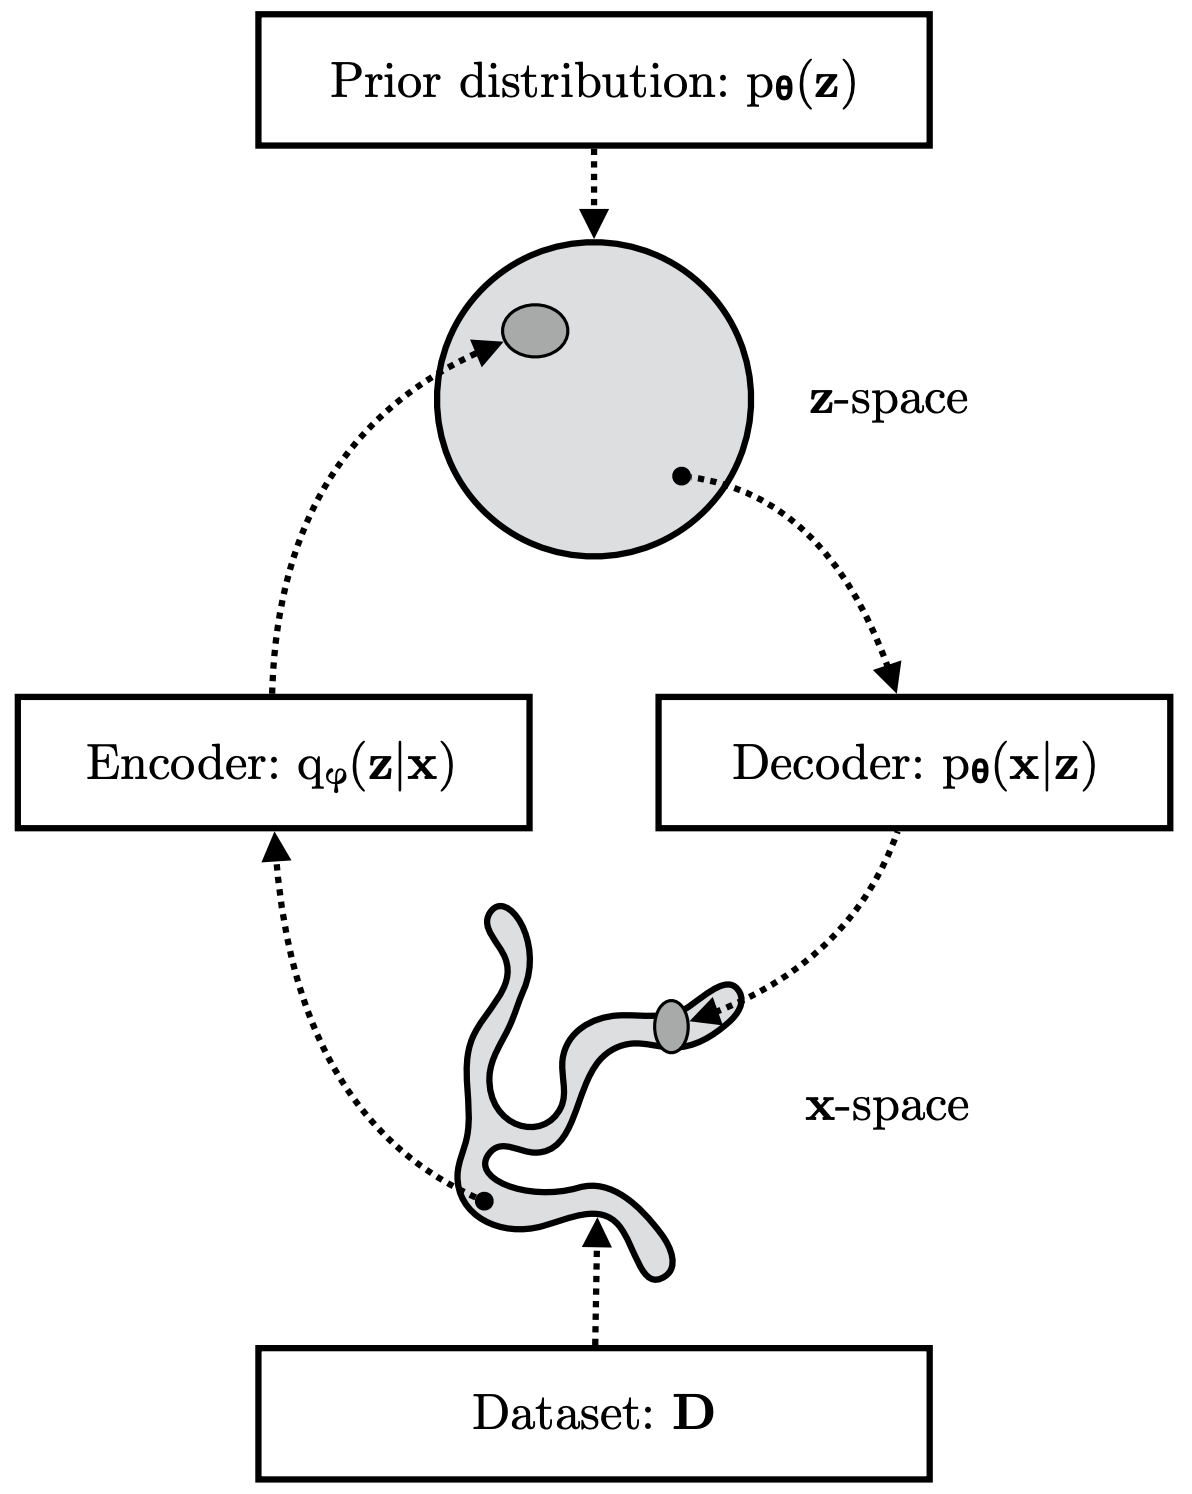
\includegraphics[width=\linewidth]{figs/vae_scheme}
		\end{figure}
	\end{minipage}
	
	\myfootnotewithlink{https://arxiv.org/abs/1906.02691}{Kingma D. P., Welling M. An introduction to variational autoencoders, 2019}
\end{frame}
%=======
\begin{frame}{Variational Autoencoder}
	\begin{figure}[h]
		\centering
		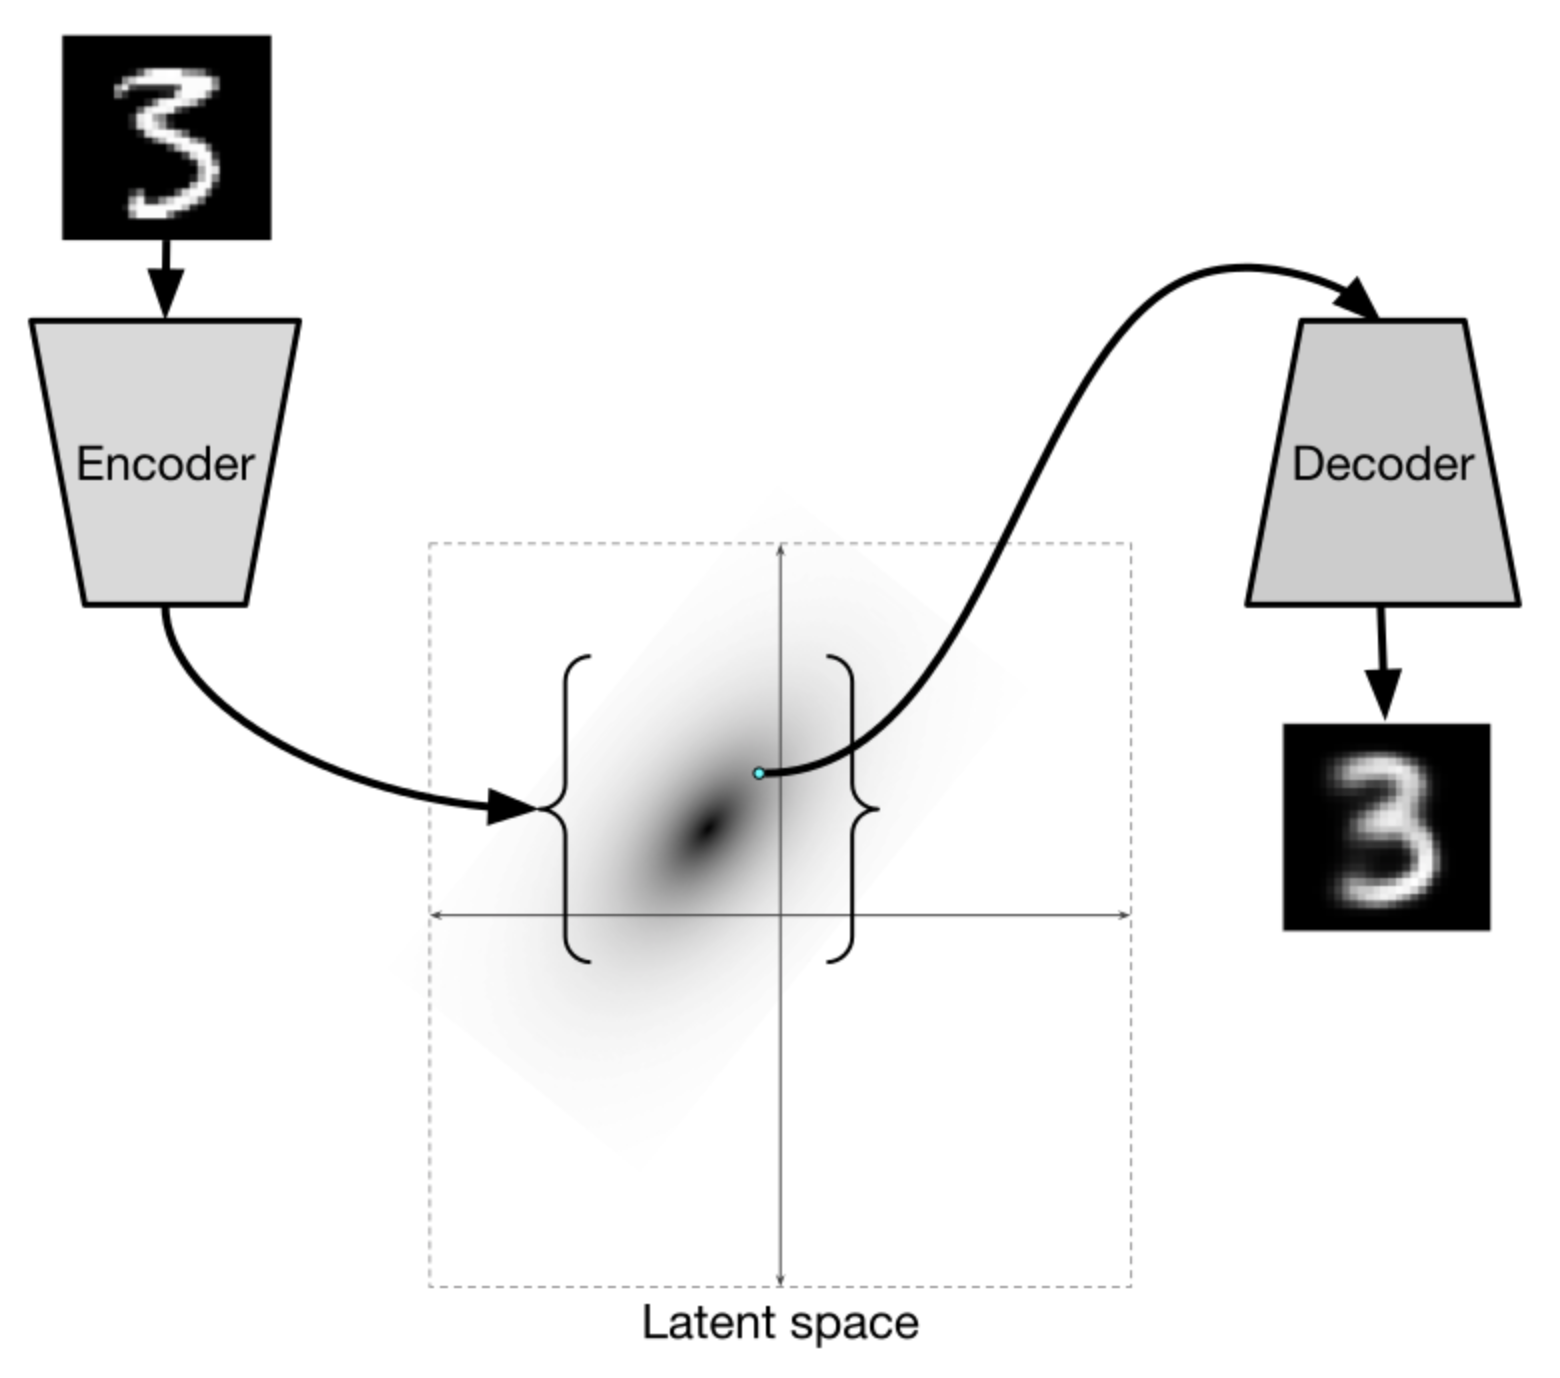
\includegraphics[width=.7\linewidth]{figs/VAE.png}
	\end{figure}
	\myfootnotewithlink{http://ijdykeman.github.io/ml/2016/12/21/cvae.html}{image credit: http://ijdykeman.github.io/ml/2016/12/21/cvae.html}
\end{frame}
%=======
\begin{frame}{Variational autoencoder (VAE)}
	\begin{itemize}
		\item Encoder $q(\bz | \bx, \bphi) = \text{NN}_e(\bx, \bphi)$ outputs $\bmu_{\bphi}(\bx)$ and $\bsigma_{\bphi}(\bx)$.
		\item Decoder $p(\bx | \bz, \btheta) = \text{NN}_d(\bz, \btheta)$ outputs parameters of the sample distribution.
	\end{itemize}
	\begin{figure}[h]
		\centering
		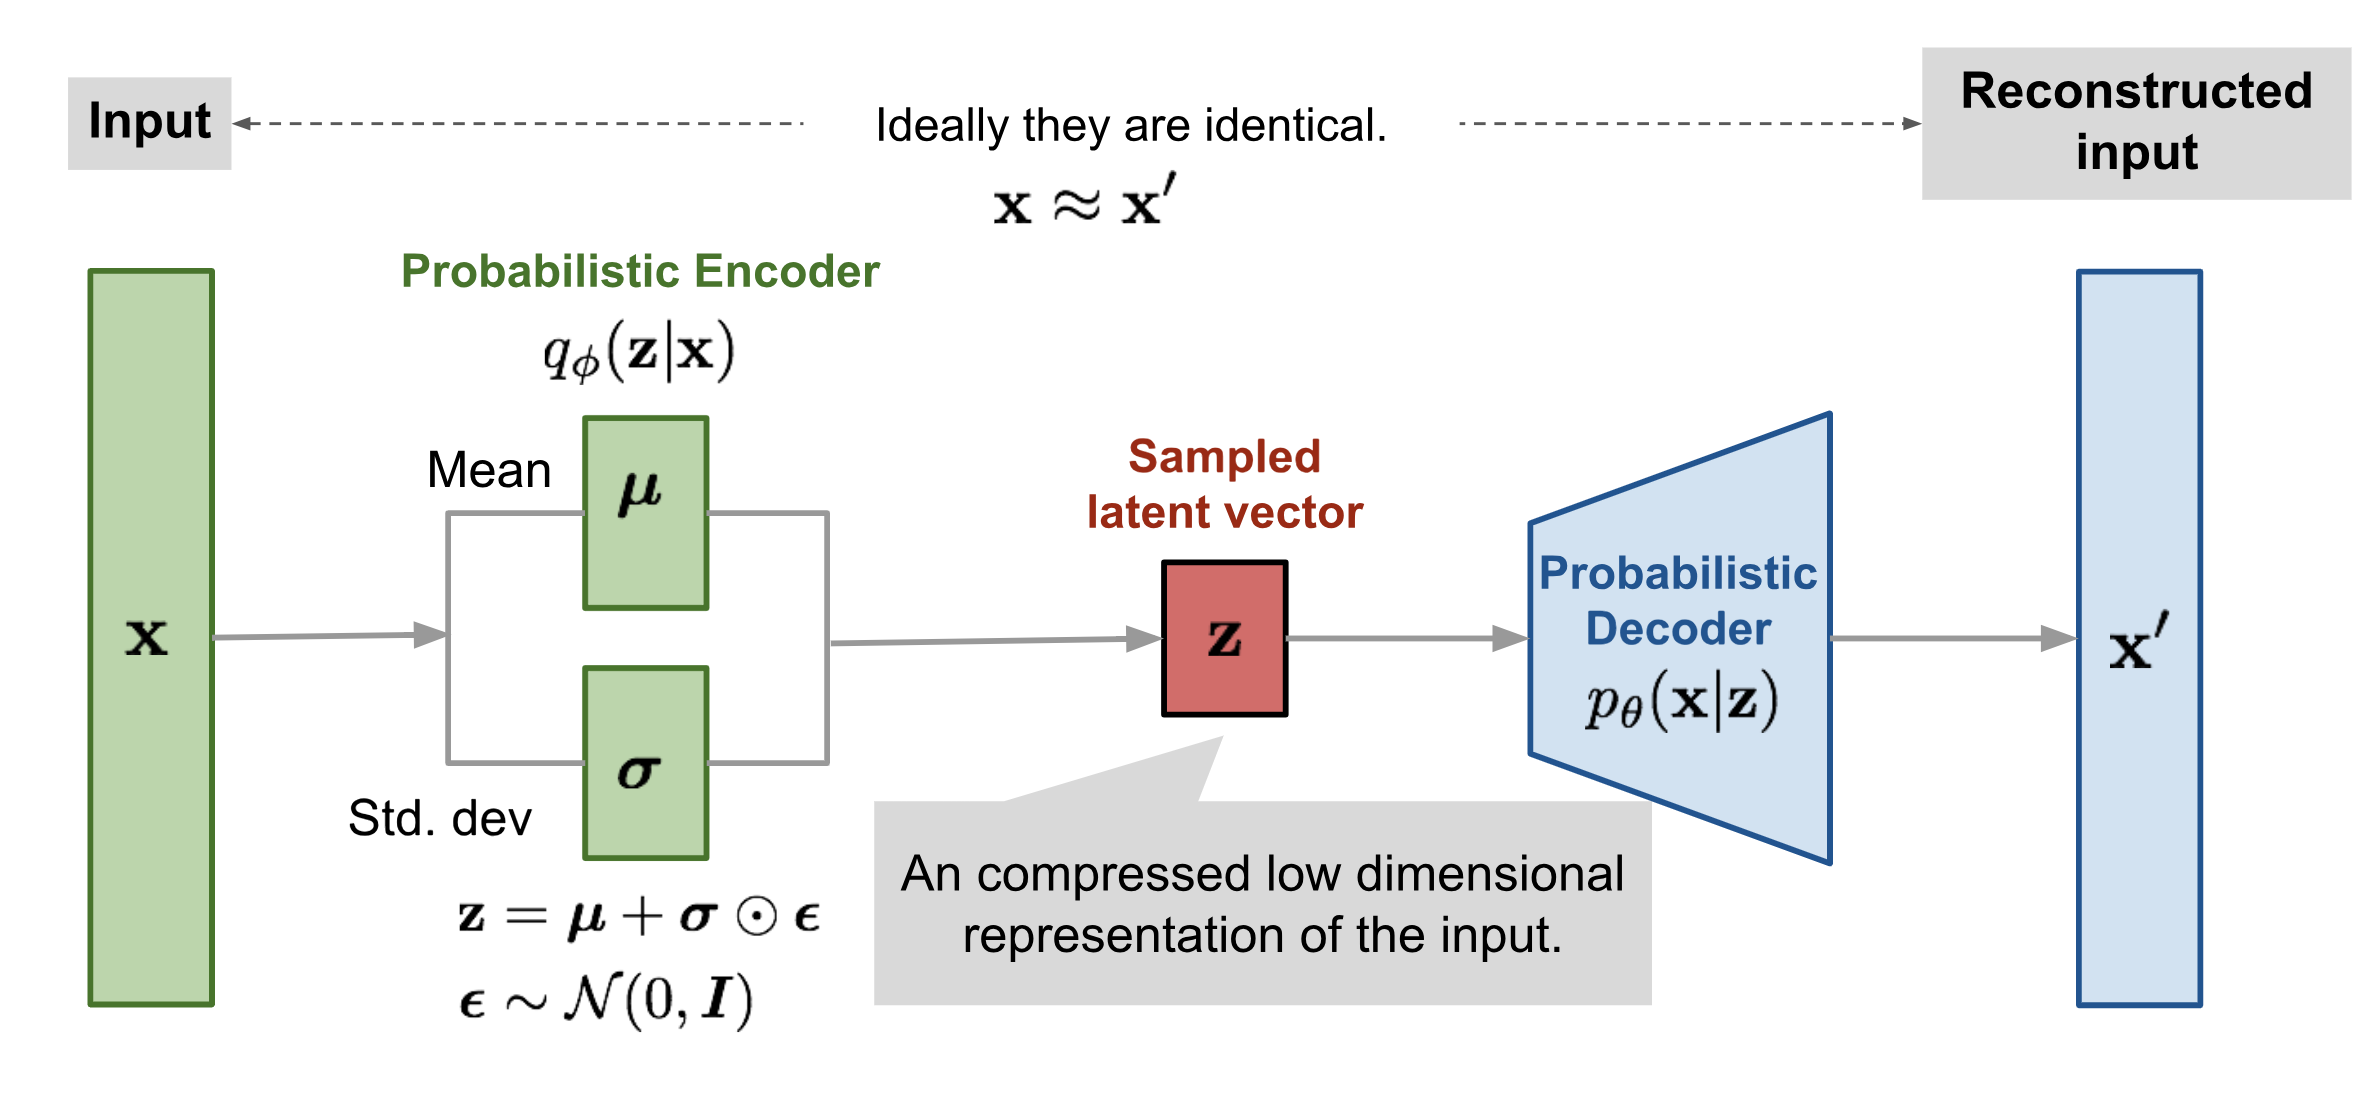
\includegraphics[width=\linewidth]{figs/vae-gaussian.png}
	\end{figure}
	
	\myfootnotewithlink{https://lilianweng.github.io/lil-log/2018/08/12/from-autoencoder-to-beta-vae.html}{image credit: https://lilianweng.github.io/lil-log/2018/08/12/from-autoencoder-to-beta-vae.html}
\end{frame}
%=======
\begin{frame}{Bayesian framework}
	\begin{block}{Posterior distribution}
		\vspace{-0.2cm}
		\[
			p(\btheta | \bX) = \frac{p(\bX | \btheta) p(\btheta)}{p(\bX)} = \frac{p(\bX | \btheta) p(\btheta)}{\int p(\bX | \btheta) p(\btheta) d \btheta} 
		\]
		\vspace{-0.2cm}
	\end{block}
	\begin{block}{Bayesian inference}
		\vspace{-0.3cm}
		\[
			p(\bx | \bX) = \int p(\bx | \btheta) p(\btheta | \bX) d \btheta
		\]
	\end{block}
    \begin{block}{Maximum a posteriori (MAP) estimation}
	    \vspace{-0.3cm}
	    \[
	        \btheta^* = \argmax_{\btheta} \log p(\btheta | \bX) = \argmax_{\btheta} \bigl(\log p(\bX | \btheta) + \log p(\btheta) \bigr)
	    \]
        \vspace{-0.3cm}
    \end{block}
	\begin{block}{MAP inference}
		\vspace{-0.4cm}
		\[
			p(\bx | \bX) = \int p(\bx| \btheta) p(\btheta | \bX ) d \btheta =  \int p(\bx| \btheta) \delta (\btheta - \btheta^* ) d \btheta \approx p(\bx | \btheta^*).
		\]
	\end{block}
\end{frame}
%=======
\begin{frame}{VAE as Bayesian model}
	\begin{block}{Posterior distribution}
		\vspace{-0.2cm}
		\[
			p(\btheta | \bX) = \frac{p(\bX | \btheta) p(\btheta)}{p(\bX)}
		\]
		\vspace{-0.5cm}
	\end{block}
	\begin{block}{ELBO}
		\vspace{-0.5cm}
		\begin{align*}
			 \log p(\btheta | \bX) &= \log p(\bX | \btheta) + \log p(\btheta) - \log p(\bX) \\
			 &= \cL(q, \btheta) + KL(q || p) + \log p(\btheta) - \log p(\bX) \\
			 &\geq \left[ \cL(q, \btheta) + \log p(\btheta) \right] - \log p(\bX) .
		\end{align*}
		\vspace{-0.7cm}
	\end{block}
	\begin{block}{EM-algorithm}
		\begin{itemize}
			\item E-step
				\vspace{-0.2cm}
				\[
					q(\bz) = \argmax_q \mathcal{L} (q, \btheta^*) = \argmin_q KL(q || p) =
				 p(\bz| \bx, \btheta^*);
				\]
				\vspace{-0.5cm}
			\item M-step
				\[
					\btheta^* = \argmax_{\btheta} \left[ \mathcal{L} (q, \btheta) + \log p(\btheta) \right].
				\]
		\end{itemize}
	\end{block}
\end{frame}
%=======
\begin{frame}{Summary}
	\begin{itemize}
		\item LVM introduces latent representation of observed samples to make model more interpretable.
		\vfill
		\item LVM maximizes variational evidence lower bound (ELBO) to find MLE of model parameters.
		\vfill
		\item The general variational EM algorithm maximizes ELBO objective.
		\vfill
		\item Amortized inference allows to efficiently compute stochastic gradients for ELBO using Monte-Carlo estimation.
		\vfill
		\item The reparametrization trick gets unbiased gradients w.r.t to a variational posterior distribution.
		\vfill
		\item The VAE model is an LVM with two neural network: for stochastic encoder $q(\bz | \bx, \bphi)$ and for stochastic decoder $p(\bx | \bz, \btheta)$.
		\vfill
		\item VAE is not a "true" bayesian model since parameters $\btheta$ do not have a prior distribution.
	\end{itemize}
\end{frame}
%=======
\end{document} 